\chapter{Durchführung}\label{chap:Durchführung}
Diese Bachelorarbeit basiert auf den Vorleistungen des Bachelorprojekts von Leander Marius Bürkin.

\section{Bachelorprojekt von Leander Bürkin}
Ziel dieses Bachelorprojekts war eine Reihe an Deutschlandkarten in einem Video zusammenzufassen, welches die Ausbreitung der COVID-19 Pandemie in Deutschland vom ersten März 2020 bis zum letzten Tag, für den die API des RKIs Daten liefert, darstellt.

\subsection{Ergebniss}
Das fertige Videos ist verfügbar unter \todo{Video verlinken}.\\
Die vom Program ausgegebene Reihe an Bilddateien wurde mithilfe des Windows Video Editors erstellt.
\\
\todo{sieben Tages Inzidenz erklären}
Die Farbe jedes Landkreises repräsentiert die sieben Tage Inzidenz des Landkreises gemäß der Legende.\\
Eine Reihe von Histogramen auf der rechten Seite zeigt die Verteilung der sieben Tage Inzidenzen alles deutschen Landkreise. Ein Histogram besteht aus 15 Säulen, wobei jede Säule einen Inzidenzbereich von 25 abdeckt. Die letzte Säule enthält zusätzlich alle sieben Tages Inzidenzen größer 350 Fälle pro sieben Tage und 100.000 Einwohner. Die Höhe der Säule entspricht jeweils der Anzahl an Landkreisen mit einer sieben Tages Inzidenz im angegebenen Bereich.

\subsection{Programmdateien}
Im Anhang finden sich die drei Programmdateien, aus denen sich sich das Programm zusammensetzt: \todo{link project files}
\todo{bild und link von video einbetten}

Die Dateien haben eine hierarchische Struktur:\\
Die Datei \glqq{}plot\_data.ipynb\grqq{} führt die Datei \glqq{}get\_data.ipynb\grqq{} aus,
welche wiederum die Datei \glqq{}get\_geographical\_data\_of\_german\_counties.ipynb\grqq{} ausführt.

Die Datei \glqq{}plot\_data.ipynb\grqq{} speichert die Grafiken schlussendlich\\
in den Ordner \glqq{}media\grqq{}.

Die Datei \glqq{}get\_data.ipynb\grqq{} konvertiert \glqq{}unpolierte\grqq{} Daten zu \glqq{}polierten\grqq{} Daten.

\glqq{}Unpolierte\grqq{} Daten sind rohe Daten direkt vom RKI oder ein Backup von diesen Daten.

Daten, die rudimentär auf Vollständigkeit überprüft wurde und bei welcher überflüssige Informationen entfernt wurde, werden \glqq{}polierte\grqq{} Daten genannt.\\
Die Datei \glqq{}get\_geographical\_data\_of\_german\_counties.ipynb\grqq{} ist ein ausgelagerter Teil von der Datei \glqq{}get\_data.ipynb\grqq{}, welcher die Informationen über die Form und die Lage der deutschen Landkreise beschafft. Dieser Vorgang nimmt überdurchschnittlich viel Platz ein, da die Form von circa 100 Landkreisen von Hand überprüft werden muss.

\subsection{Daten}
\subsubsection{Format und Aufteilung der Daten}
Die Daten liegen in einer Kombination aus Python Dictionaries und Python Listen vor. Ein Dictionary ist dadurch charakterisiert, dass man über den Namen eines Elements (der \glqq{}Key\grqq{}) das Element bekommt, ähnlich der Adresse bei einem Haus. Listen sind dadurch charakterisiert, dass sie Elemente in einer fixen Reihenfolge enthalten und sich diese durch ihren Index leicht ausfindbar machen. So sind beispielsweise die Anzahl der COVID-19 Fälle der einzelnen Tage chronologisch in einer Liste gespeichert, sodass man daraus direkt eine Abbildung erstellen kann.\ \\
Die Programmdateien erstellen drei verschiedene Dictionaries, welche (in untergeordneten Dictionaries und Listen) alle Daten enthalten:
\begin{itemize}
    \item covid19
    \item counties\_geography
    \item non\_county\_specific\_data
\end{itemize}

\textbf{covid19}\\
Das Dictionary covid19 speichert die COVID-19 Fälle jedes deutschen Landkreises und die daraus berechnete sieben Tages Inzidenz.

Mit dem Gemeindeschlüssel eines Landkreises als Key und dem zusätzlichen Key \glqq{}cases\grqq{} erhält man die akkumulierte Anzahl an COVID-19 Fällen pro Tag des Landkreises als Liste.

Mit dem Gemeindeschlüssel eines Landkreises als Key und dem Key \glqq{}incidences\grqq{} erhält man die sieben Tages Inzidenz pro Tag des Landkreises als Liste.

Beide Listen enthalten für jeden Tag seit dem 01.03.2020 bis zu dem Tag der aktuellsten Daten jeweils einen Eintrag.

Die Anzahl an COVID-19 Fällen pro Tag stamt aus dem \glqq{}COVID-19 Datenhub\grqq{} (https://npgeo-corona-npgeo-de.hub.arcgis.com/). Die sieben Tages Inzidenz wurde aus den Daten vom COVID-19 Datenhub berechnet.

\textbf{counties\_geography}\\
Das Dictionary counties\_geography enthält zu jedem Landkreis ein Dictionary mit den folgenden Elemente:
\begin{itemize}
    \item[name:] Der Name des Landkreises
    \item[population:] Die Einwohnerzahl des Landkreis aus einer offiziellen Schätzung (nähere Informationen finden sich im COVID-19 Datenhub). Diese Zahlen werden auch für die offizielle Berechnung der sieben Tages Inzidenz verwendet.
    \item[area\_in\_m2:] Die Fläche des Landkreises in Quadratmetern
    \item[geometry:] Die Form des Landkreises in einer für die Darstellung angepassten Form
    \item[raw\_geometry:] Die Form des Landkreises in der originalen Form
    \item[population\_density:] Die Bevölkerungsdichte des Landkreises, berechnet aus der Fläche des Landkreises und seiner Einwohnerzahl
\end{itemize}
Außer die Bevölkerungsdichte, welche berechnet wird, und die angepassten Formen der Landkreise, welche aus den origialen Formen generiert werden, stammen alle Daten direkt aus dem \glqq{}COVID-19 Datenhub\grqq{} (https://npgeo-corona-npgeo-de.hub.arcgis.com/).

\textbf{non\_county\_specific\_data}
Das Dictionary non\_county\_specific\_data enthält die folgenden Elemente:
\begin{itemize}
    \item[unixtime:] Die Unixzeit, wie sie vom COVID-19 Datenhub zur Verfügung gestellt wird: Die Zahl der Millisekunden seit dem 01.01.1970 00:00 Uhr UTC. Die Zahl der COVID-19 Fälle und die sieben Tages Inzidenz eines entsprechenden Tages befinden sich an der selben Stelle in Ihrer jeweiligen Liste, wie der Tag in dieser Liste.
    \item[states:] Die Name und Nummern der deutschen Bundesländer. Die ersten beiden oder die erste Zahl des Gemeindeschlüssel eines Landkreises repräsentiert das Bundesland, in welchem der Landkreis liegt.
    \item[highest\_case\_number:] Die höchste akkumulierte Fallzahl unter allen Landkreisen.
    \item[lowest\_case\_number:] Die niedrigste akkumulierte Fallzahl unter allen Landkreisen.
    \item[highest\_incidence:] Die höchste sieben Tages Inzidenz eines Tages unter allen Landkreisen.
    \item[lowest\_incidence:] Die niedrigste sieben Tages Inzidenz eines Tages unter allen Landkreisen.
    \item[UTC:] Die Unixzeit konvertiert in die Koordinierte Weltzeit \glqq{}DD.MM.YYYY\grqq{}.
    \item[UTC+7days:] Die Liste der Zeiten gespeichert in UTC plus sieben Tage vor dem erstem Datum in der Liste, um den Zeitraum der sieben Tages Inzidenz der ersten sieben Tage darstellen zu können: die hierfür verwendeten Zeiträume beginnen jeweils vor dem ersten hier dokumentierten Fall.
\end{itemize}
Die Unixzeit, die Namen und die Nummern der Bundesländer stammen aus dem \glqq{}COVID-19 Datenhub\grqq{} (https://npgeo-corona-npgeo-de.hub.arcgis.com/). Alle anderen Informationen wurden gesammelt oder berechnet.

In Abbildung \ref{fig:dicts_als_code} sind die drei Dictionaries dargestellt, wie sie auch im Programm verwendet werden.
\begin{figure}[H]
    \centering
    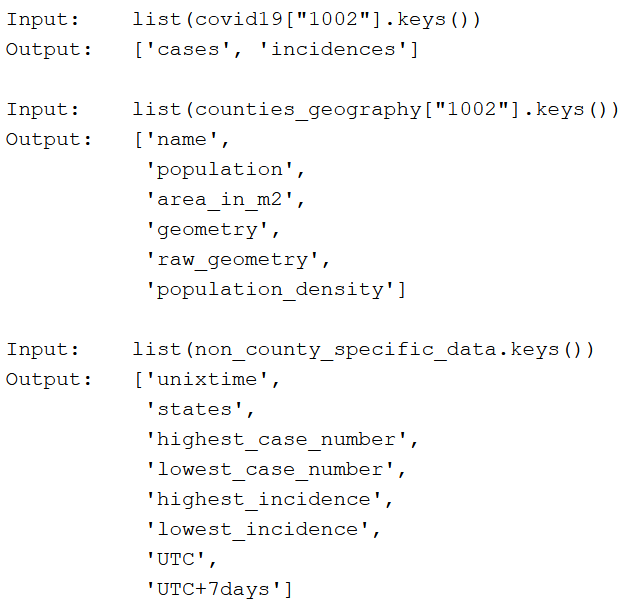
\includegraphics[width=0.8\textwidth]{figures/Durchführung/Dictionarys Bachelorprojekt.png}
    \caption{
    Die Dictionaries non\_county\_specific\_data, counties\_geography und covid19 mit ihren jeweiligen Schlüsseln.
    Für die Dictionaries covid19 und counties\_geography wurde jeweils der Landkreis Kiel (Gemeindeschlüssel 1002) zur Veranschaulichung verwendet.}
    \label{fig:dicts_als_code}
\end{figure}


\subsubsection{Datenquellen - Ursprung und Abspeicherung}
Das Bachelorprojekt verwendet Informationen zur COVID-19 Pandemie und den geographischen Daten von 412 deutschen Landkreisen. Alle Daten stammen aus dem \glqq{}COVID-19 Datenhub\grqq{} (https://npgeo-corona-npgeo-de.hub.arcgis.com/) oder wurden aus den daher stammenden Daten generiert. Diese Datenquelle wurde gewählt, weil sie vom Robert-Koch-Institut (RKI, www.rki.de) und dem deutschen Staat referenziert wird.\todo{Staat refernzieren}

Die Daten sind in drei verschiedenen Formen gespeichert:
\begin{itemize}
    \item Als originale Daten auf dem Server des RKIs, erreichbar durch eine sogenannte API.
    \item Als unpolierte Daten auf der Maschine, welche das Program ausführt, als Backup, wenn die API nicht erreichbar ist.
    \item Als polierte Daten auf der Maschine, welche das Program ausführt, für den sofortigen Gebrauch.
\end{itemize}
\todo{Vergleiche mit (kommentar siehe Code)}
% https://www.rki.de/DE/Content/Infekt/EpidBull/Archiv/2020/Ausgaben/17_20.pdf?__blob=publicationFile

\section{Einordnung und weitere Visualisierung der Daten}
Im folgenden wird die Korrelation der Corona-Fälle der einzelnen deutschen Landkreise untersucht. Um dieses Verfahren besser zu verstehen und ein grobes Gefühl für den Datensatz zu bekommen, werden die einzelnen Werte gesondert an.

\subsection{Die deutschen Landkreise und Ihre Bevölkerungsdichte}
Zuallererst folgen die genutzten Daten, welche nichts mit Corona zutun haben: Die Landkreise und ihre Bevölkerungsdichte. Die Bevölkerungsdichte wird aus der Bevölkerungszahl und der Fläche des Landkreises berechnet, welche von der API bereitgestellt werden \todo{adäquate Verlinkung auf API}.

In Abbildung \autoref{fig:distribution_pop_density_counties} sind die Bevölkerungsdichten der einzelnen Landkreise dargestellt. Auf der linken Seite befindet sich die Verteilung und auf der rechten Seite die räumliche Anordnung.
Die Bezirke Berlins sind einzeln gelistet, daher entsprechen die sechs höchsten Bevölkerungsdichten den Berliner Bezirken  Friedrichshain-Kreuzberg, Mitte, Neukölln, Tempelhof-Schöneberg, Lichtenberg, Charlottenburg-Wilmersdorf, obwohl die Bevölkerungsdichte des gesamten Berliner Stadtkreises niedriger ist als die Bevölkerungsdichte Münchens (in dieser Auflistung Platz 7, ohne Berliner Bezirke Platz 1).

\begin{figure}[H]
    \centering
    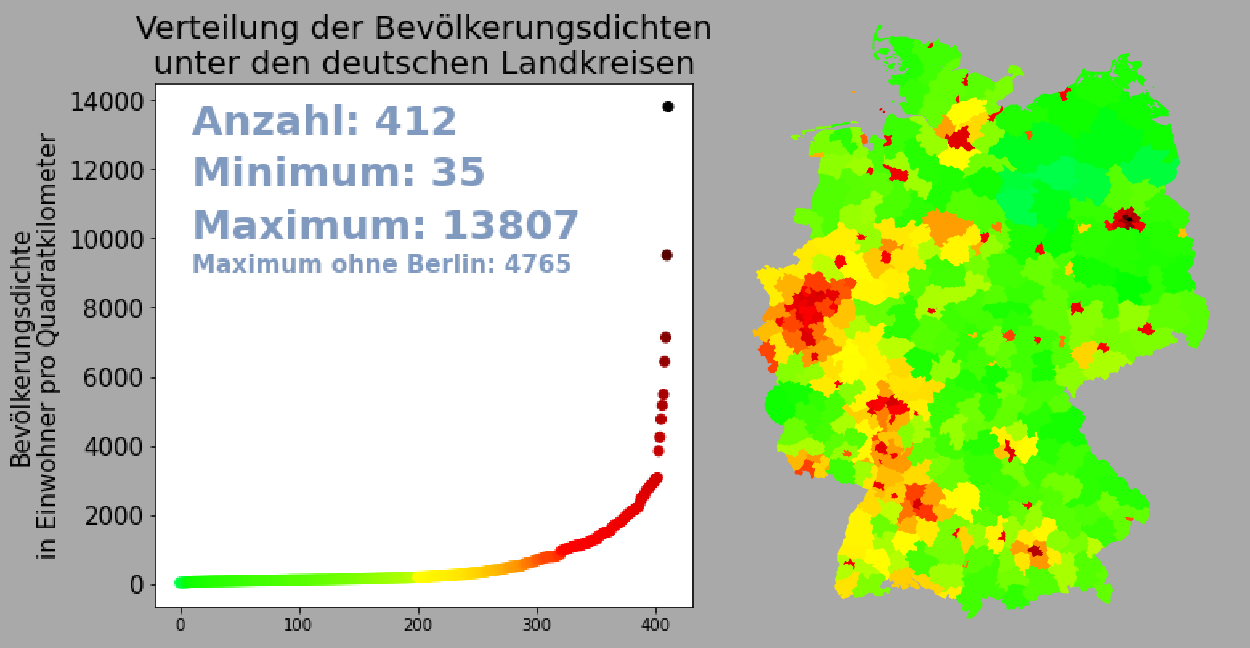
\includegraphics[width = 0.95\textwidth]{figures/Durchführung/population_density_counties_Distribution_and_map.png}
    \caption{Verteilung der Bevölkerungsdichten unter den deutschen Landkreisen.}
    \label{fig:distribution_pop_density_counties}
\end{figure}

\todo{klarstellen, das die Landkreise nicht den Landkreisen entsprechen (Berlin ist aufgeteilt) Aus Wikipedia "Landkreis": In Deutschland gibt es 294 Landkreise. Zusammen mit den 106 kreisfreien Städten bilden sie die insgesamt 400 Gebietskörperschaften auf Kreisebene. Wir haben 412.}
In Abbildung 


Teilt man die Landkreise nach den ersten beiden Kennzahlen des Landkreises, die des Bundeslandes und die des aktuellen (teils auch vergangenen) Regierungsbezirks, ein, ergibt sich für die Bevölkerungsdichte das in \autoref{fig:distribution_pop_density_districts} dargestellte Bild.

Nicht alle Bundesländer wurden in Regierungsbezirke unterteilt, in diesem Fall wird die Bevölkerungsdichte des Landkreises gewählt. Im folgenden wird dennoch von \glqq{}den Regierungsbezirken\grqq{} gesprochen. Zudem sind die Stadtstaaten Bremen und Hamburg zum Regierungsbezirk Lüneburg hinzugefügt und der Stadtstaat Berlin zum Bundesland Brandenburg hinzugefügt.

\begin{figure}[H]
    \centering
    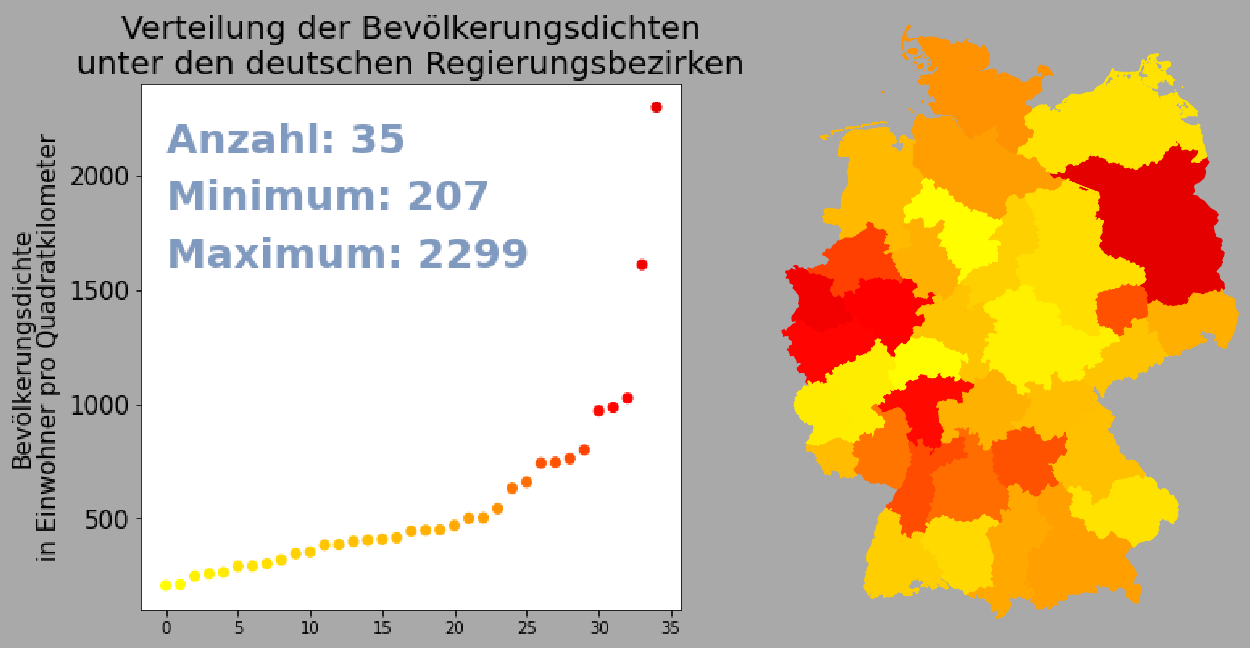
\includegraphics[width = 0.95\textwidth]{figures/Durchführung/population_density_districts_Distribution_and_map.png}
    \caption{Verteilung der Bevölkerungsdichten unter den deutschen Regierungsbezirken. Die Skalierung entspricht der Farbgebung in \autoref{fig:distribution_pop_density_counties}.}
    \label{fig:distribution_pop_density_districts}
\end{figure}

Klar zu erkennen sind die Stadtkreise in Abbildung \ref{fig:distribution_pop_density_counties}: Sie weisen eine hohe Bevölkerungsdichte auf und sind in der Regel von weniger stark bevölkerten Landkreisen umgeben.

Die Städte in Tabelle \ref{tab:landkreise_um_städte} von einem Landkreis umgeben, an Ihnen lässt sich besonders gut testen, ob sich in den Korrelationswahrscheinlichkeiten zwischen einer Stadt und ihrem Umland eine zeitliche Verschiebung feststellen lässt.
\begin{table}[H]
    \centering
    \begin{tabular}{c}
Kassel 6633\\
Trier-Saarburg 7235\\
Südliche Weinstraße 7337\\
Südwestpfalz 7340\\
Heilbronn 8125\\
Rastatt 8216\\
Rosenheim 9187\\
Landshut 9274\\
Straubing-Bogen 9278\\
Amberg-Sulzbach 9371\\
Beustadt a.d. Waldnaab 9374\\
Regensburg 9375\\
Bamberg 9471\\
Bayreuth 9472\\
Coburg 9473\\
Hof 9475\\
Ansbach 9571\\
Schweinfurt 9678\\
Würzburg 9679\\
Ostallgäu 9777\\
Oberallgäu 9780\\
Potsdam-Mittelmark 12069\\
Spree-Neiße 12071\\
Saalekreis 15088\\
Weimarer Land 16071\\
\todo{fill table}
    \end{tabular}
    \caption{Landkreise mit Name und Gemeindeschlüssel, die eine Stadt komplett umgeben.}
    \label{tab:landkreise_um_städte}
\end{table}
Als erstes Beispiel zu Demonstrationszwecken ausführlich gezeigt.

